\section{Stabilität von MOS Operationsverstärker}
\begin{figure}[!h]
	\centering
	\begin{subfigure}[b]{10cm}
		\centering
		\adjustbox{scale=0.8}{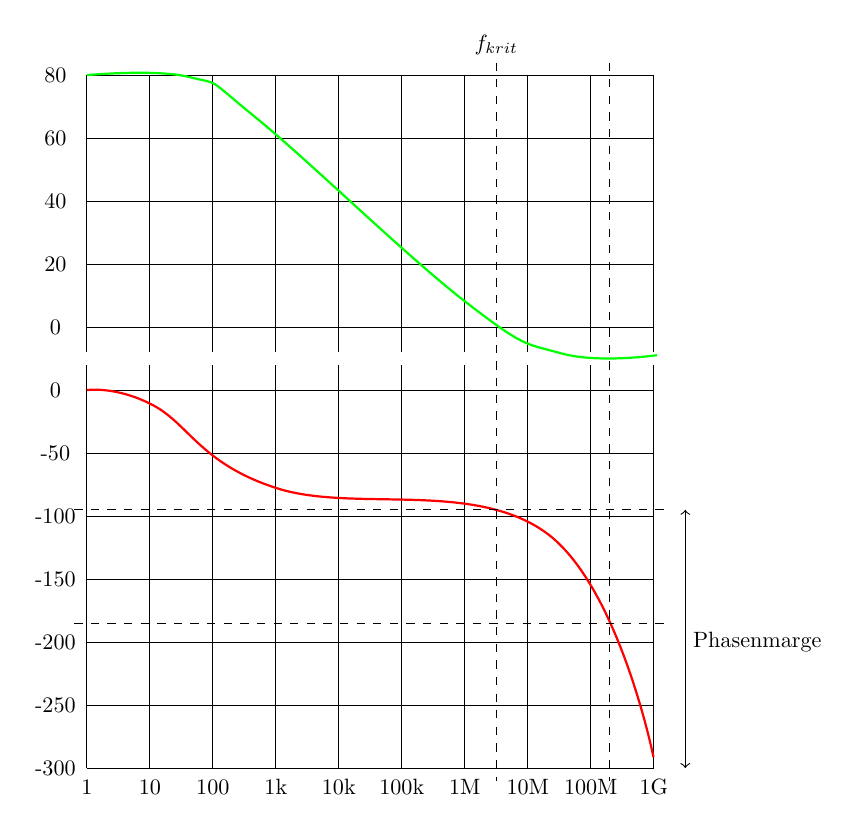
\begin{tikzpicture}[scale=0.8,transform shape]
	%axis
	%x
	\foreach \x in {0,...,9} {
		\draw (\x,0) -- (\x,6.4);
		\draw (\x,6.6) -- (\x,11);
	}
	%y
	\foreach \y in {0,...,11} {
		\draw (0,\y) -- (9,\y);
	}
	\draw node at (0,-0.3) {1};
	\draw node at (1,-0.3) {10};
	\draw node at (2,-0.3) {100};
	\draw node at (3,-0.3) {1k};
	\draw node at (4,-0.3) {10k};
	\draw node at (5,-0.3) {100k};
	\draw node at (6,-0.3) {1M};
	\draw node at (7,-0.3) {10M};
	\draw node at (8,-0.3) {100M};
	\draw node at (9,-0.3) {1G};
	
	\draw node at (-0.5,0) {-300};
	\draw node at (-0.5,1) {-250};
	\draw node at (-0.5,2) {-200};
	\draw node at (-0.5,3) {-150};
	\draw node at (-0.5,4) {-100};
	\draw node at (-0.5,5) {-50};
	\draw node at (-0.5,6) {0};
	\draw node at (-0.5,7) {0};
	\draw node at (-0.5,8) {20};
	\draw node at (-0.5,9) {40};
	\draw node at (-0.5,10) {60};
	\draw node at (-0.5,11) {80};

\draw [thick, red] plot[smooth, tension=.7] coordinates {(0,6) (1.0379,5.7673) (3.0063,4.4457) (7.2804,3.7427) (8.9957,0.1716)    };
\draw [thick, green] plot[smooth, tension=.7] coordinates {(0,11) (1.6284,10.9694) (2.697,10.314) (6.0151,7.3983) (7.5335,6.5828) (9.052,6.5547)};
\draw [dashed] (6.5,11.2) -- (6.5,-0.2);
\draw [dashed] (8.3,11.2) -- (8.3,-0.2);
\draw [dashed] (-0.2,2.3) -- (9.2,2.3);
\draw [dashed] (-0.2,4.1) -- (9.2,4.1);
\draw [<->] (9.5,4.1) -- (9.5,0);
\draw node at (9.5,2) [anchor=west] {Phasenmarge};
\draw node at (6.5,11.2) [anchor=south] {$f_{krit}$};
\end{tikzpicture}
}
		\caption{Bodeplot}
	\end{subfigure}\qquad
	\begin{subfigure}[b]{8cm}
		\centering
		{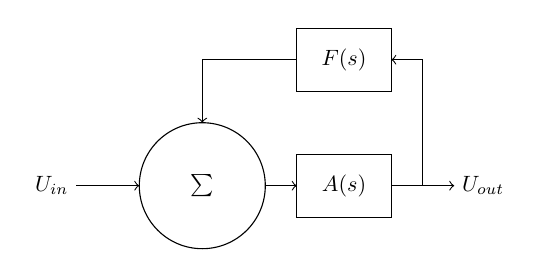
\begin{tikzpicture}[scale=0.8,transform shape]
	\draw [->] (0,0) node [anchor=east] {$U_{in}$} -- (1,0);
	\draw (2,0) circle (1);
	\draw node at (2,0) {$\sum$};
	\draw [->] (3,0) -- (3.5,0);
	\draw (3.5,0.5) rectangle (5,-0.5);
	\draw node at (4.25,0) {$A(s)$};
	\draw [->] (5,0) -- (6,0) node [anchor=west] {$U_{out}$};
	\draw [->] (5.5,0) -- (5.5,2) -- (5,2);
	\draw (5,2.5) rectangle (3.5,1.5);
	\draw node at (4.25,2) {$F(s)$};
	\draw [->] (3.5,2) -- (2,2) -- (2,1);
	

\end{tikzpicture}}
		\caption{Rückgekoppelter Verstärker}
	\end{subfigure}
	\caption{Stabilität}
	\label{fig:stabilitaet}
\end{figure}

\begin{tabular}{|l|l|}
\hline
	Phasenmarge bei $f_{krit}(a_L=1)$ &
	Verhalten des Verstärkers \\
	& (System mit zwei weit auseinanderliegenden Polen) \\\hline
	$\varphi_M \leq 0^\circ$ & 
	Gegenkoppelter Verstärker schwingt selbständig \\\hline
	$\varphi_M > 0^\circ$ &
	Gedämpftes Überschwingen der Sprungantwort \\\hline
	$\varphi_M = 65^\circ$ &
	Peaking verschwindet. Einziger Überschwinger mit 4.7\% Sprunghöhe \\\hline
	$\varphi_M \geq 75^\circ$ &
	Kein Überschwingen \\\hline
\end{tabular}

\begin{tabular}{lll}
Stabilitätskriterien & $\Phi = 180^\circ$ & $ \left|A(s)\cdot F(s)\right|<1 $ \\
& $ \left|A(s)\cdot F(s)\right|= 1 $ & $ \rightarrow 180^\circ-\Phi>0;\
\varphi_M>0^\circ $ \\
Phasenmarge & $\varphi_M=180^\circ-\Phi =90^\circ - \arctan(\frac{GBP}{f_{P2}})$ & \\
Designregel & Wähle 2. Pol ($f_{nd}$) bei ca. $3\cdot GBP$& \\
\end{tabular}